\documentclass[aspectratio=169]{beamer}
\usetheme[width=3\baselineskip]{PaloAlto}
\usecolortheme{seahorse}

\setbeamertemplate{navigation symbols}{%
    \usebeamerfont{footline}%
    \usebeamercolor[fg]{footline}%
    \hspace{1em}%
    \insertframenumber/\inserttotalframenumber
}

\usepackage{todonotes}

\makeatletter
\beamer@headheight=\beamer@sidebarwidth
\makeatother

\makeatletter
\logo{
\includegraphics[width=\beamer@sidebarwidth]{logo_transp}}
\makeatother

\usepackage{graphicx}
\graphicspath{{./img/}}
\usepackage[utf8]{inputenc}
\usepackage[english,italian]{babel}
\usepackage{listings}
\usepackage[backend=bibtex,citestyle=verbose-ibid]{biblatex}
\bibliography{biblio} 

\lstdefinelanguage{cpp}{
  language=C++,
  basicstyle=\ttfamily,
  breaklines=true,
  keywordstyle=\color{blue}\ttfamily,
  stringstyle=\color{red}\ttfamily,
  commentstyle=\color{green}\ttfamily,
  morecomment=[l][\color{magenta}]{\#}
}

\lstdefinelanguage{yaml}{ 
  basicstyle=\ttfamily,
   breaklines=true,
}

%Information to be included in the title page:
\title{CONVERSIONE DI STRUMENTI VINTAGE PER LA DATA PHYSICALIZATION}
\author{Davide Busolin}
\institute{Università degli Studi di Milano \\ Dipartimento di Informatica ``Giovanni degli Antoni"}
\date{16/07/2021}

\begin{document}

\frame{\titlepage}

\section{Contesto}

\begin{frame}[allowframebreaks]
\frametitle{Data Physicalization}
%Una data physicalization (in italiano: fisicalizzazione dei dati) è un artefatto fisico la cui geometria o proprietà materiali codificano dei dati.

\begin{figure}[h]
  \centering
  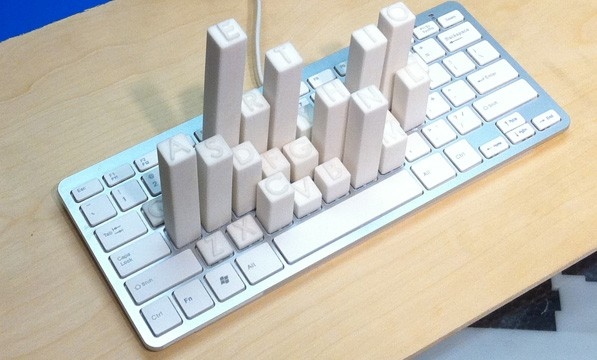
\includegraphics[width=0.6\textwidth]{keyboardfreq}
  \caption{Keyboard Frequency Sculpture\autocite{physlist}}
\end{figure}

\framebreak

\begin{figure}[h]
  \centering
  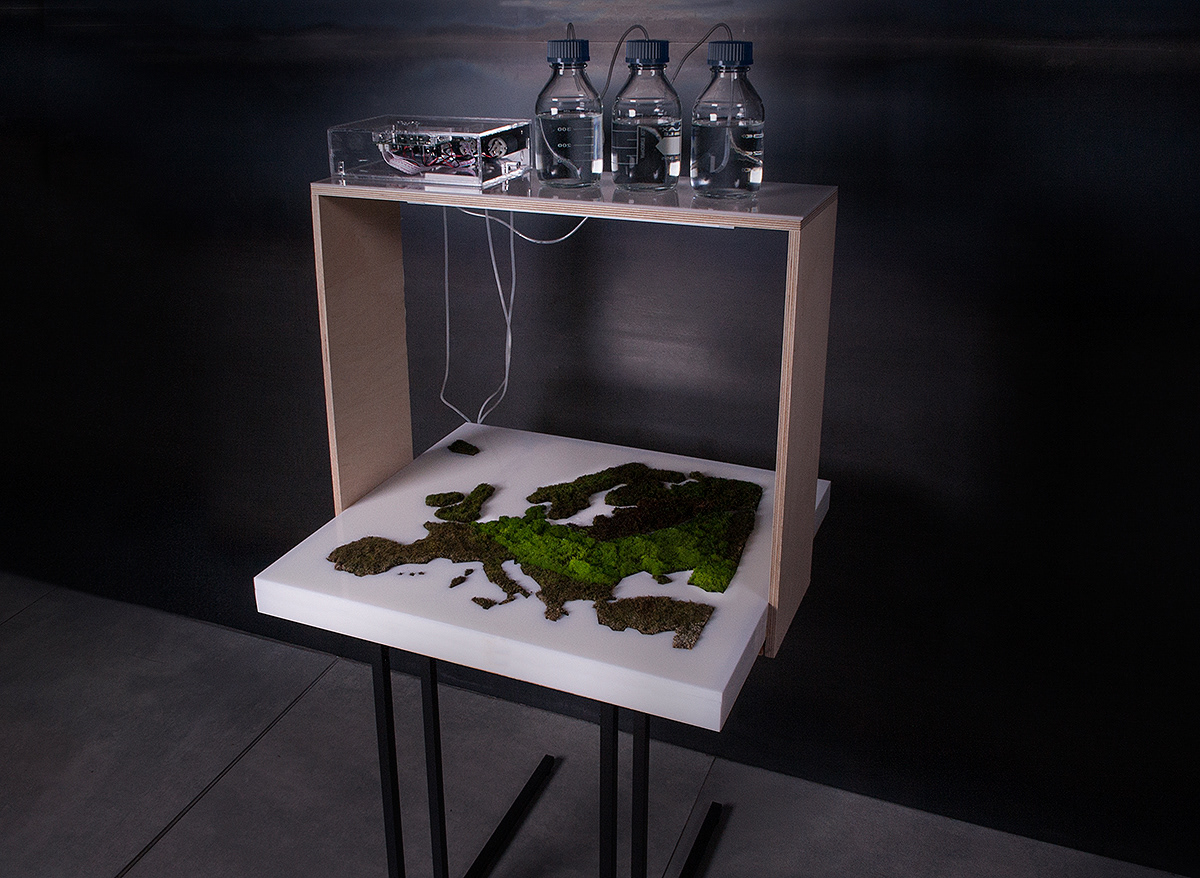
\includegraphics[width=0.5\textwidth]{livingmap}
  \caption{Living Map: Precipitation Visualized with Moss\autocite{physlist}}
\end{figure}
\end{frame}\todo{atrent: queste due le metterei in una sola}





\begin{frame}
\frametitle{Data Visualization}
%Lo scopo della disciplina della visualizzazione dei dati è quello di renderli più comprensibili per gli esseri umani.

\begin{columns}
\column{0.45\textwidth}
\onslide<1->{
  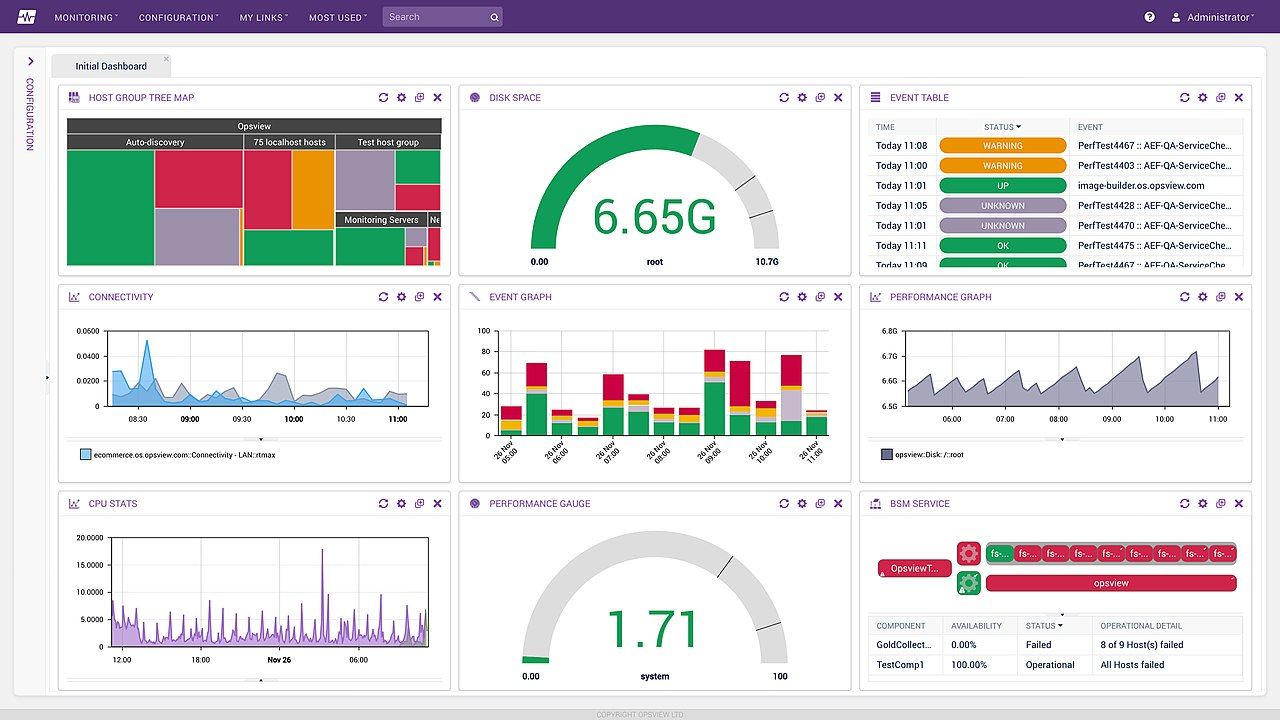
\includegraphics[width=0.95\textwidth]{datadash}\footnotemark 
}%
\onslide<2->{\column{0.1\textwidth}\centering$\rightarrow$
  \column{0.45\textwidth}
  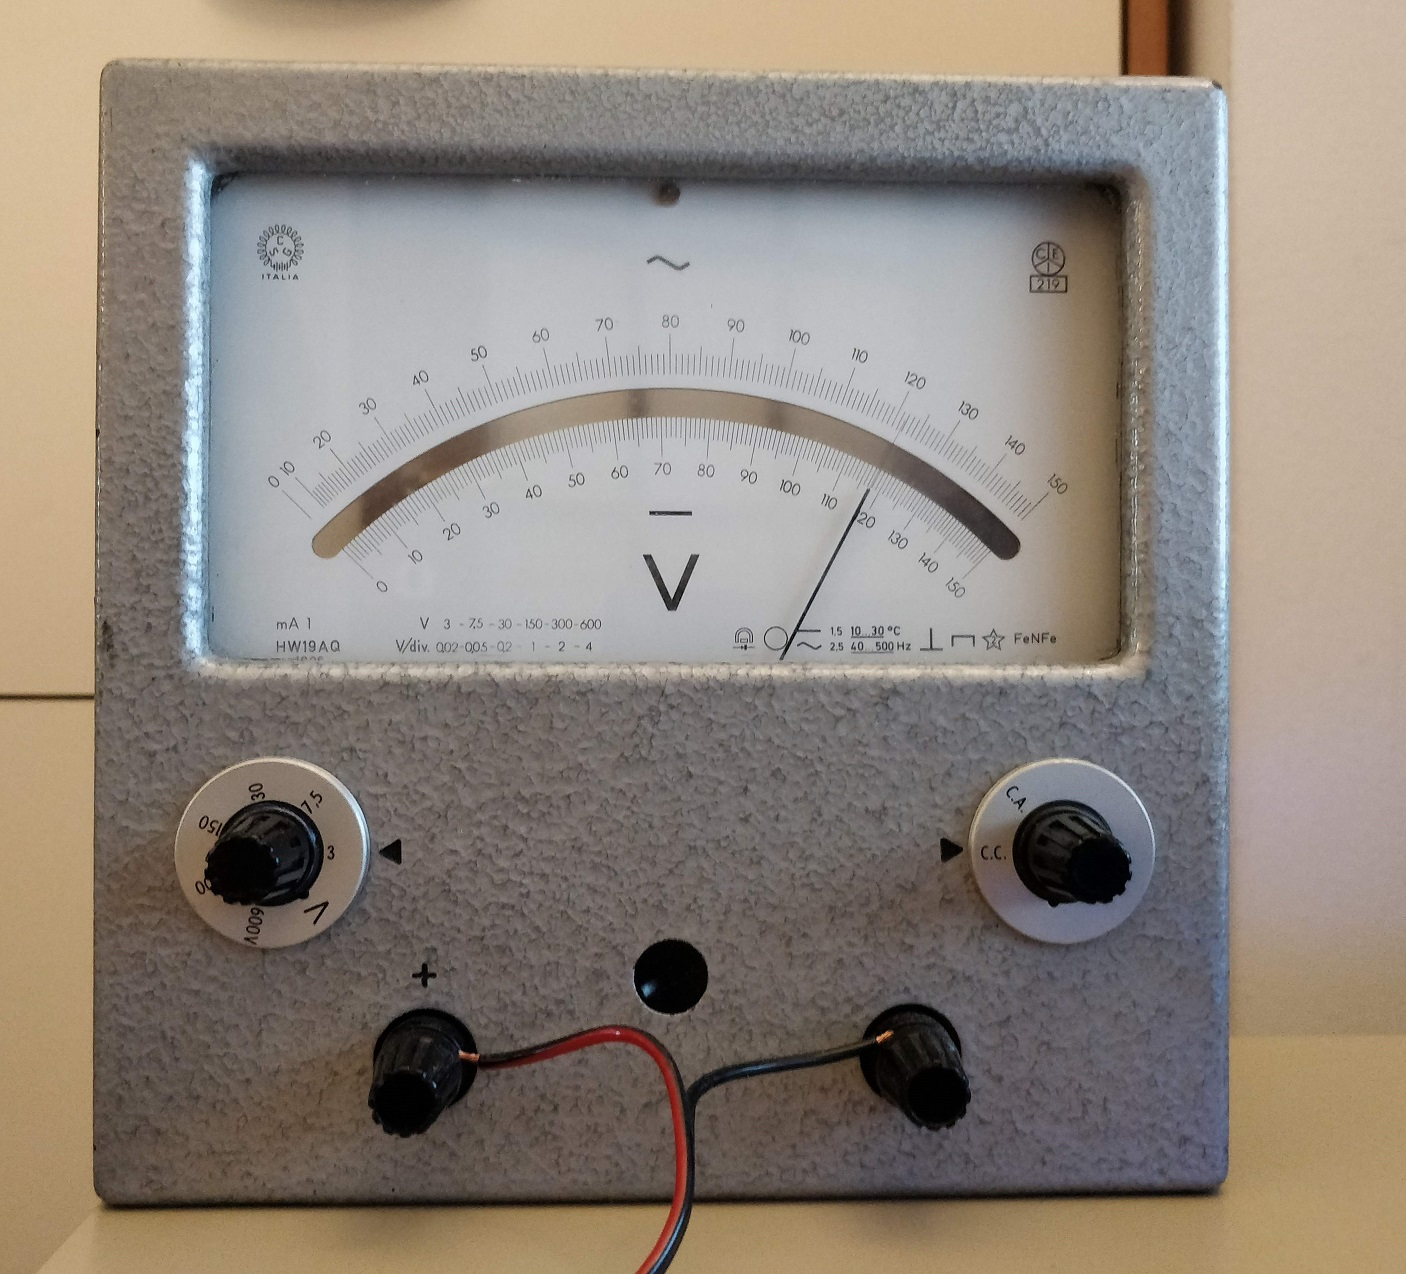
\includegraphics[width=\textwidth]{interventominimale}
}
\end{columns}

\footcitetext{wiki:datadash}
\end{frame}\todo{atrent: idem}

\section{Obiettivo}

\begin{frame}
\frametitle{Obiettivo}
Analizzare e sperimentare una forma di fisicalizzazione dei dati mediante strumenti di misura vintage e al contempo realizzare una guida alla conversione.

\end{frame}

\begin{frame}
\frametitle{ESP8266}
%https://commons.wikimedia.org/wiki/File:WeMos_D1_Mini_front.jpg
\begin{figure}[h]
  \centering
  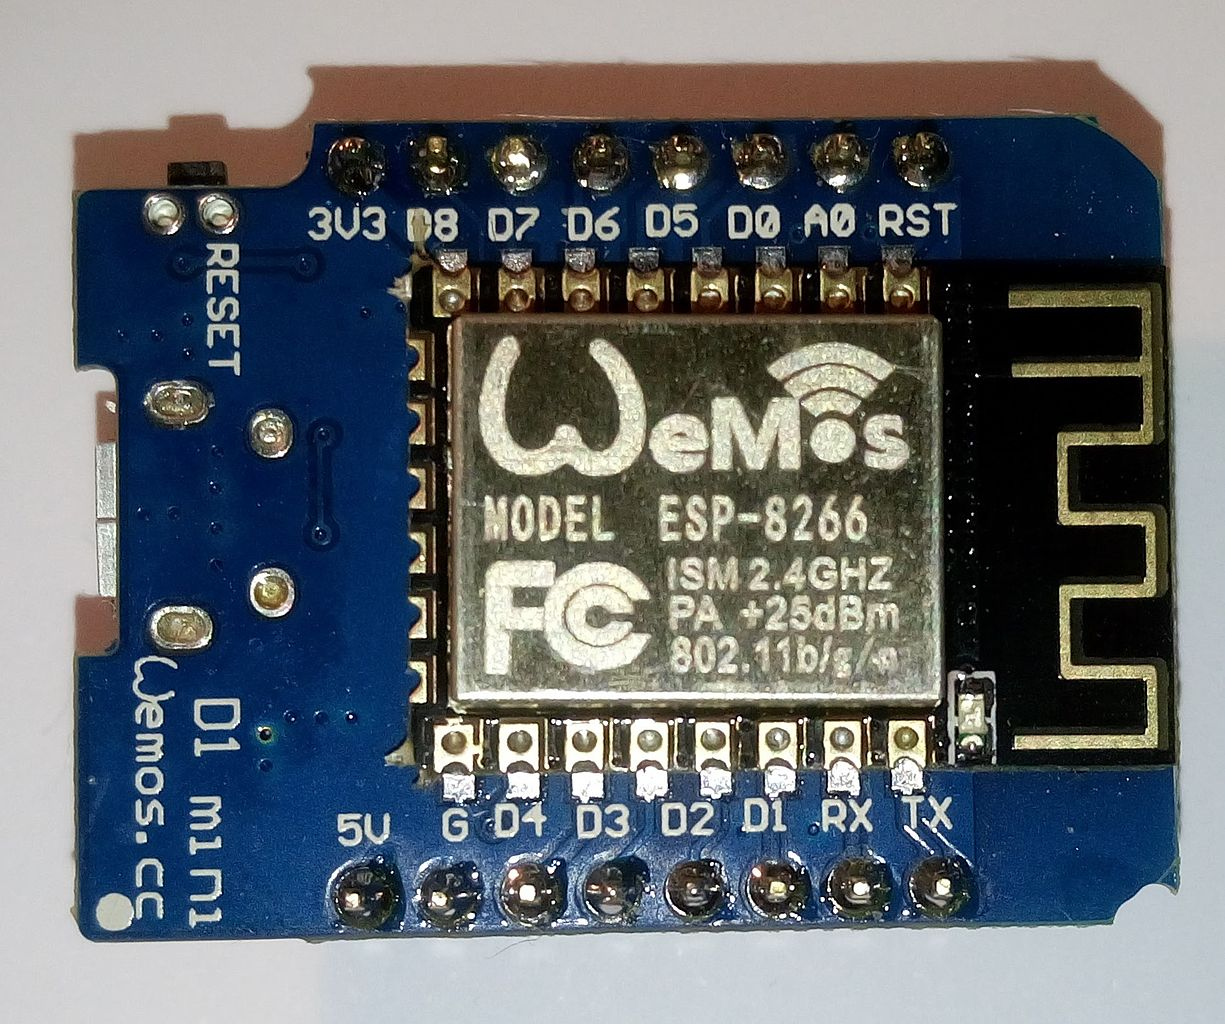
\includegraphics[width=0.4\textwidth]{wd1mini}
  \caption{WeMos D1 Mini\autocite{wiki:wd1mini}}
\end{figure}

\end{frame}

\section{Stato dell'arte}

\begin{frame}[allowframebreaks]
\frametitle{Esempi di riutilizzo di strumenti \textit{vintage}}
\begin{figure}[h]
  \centering
  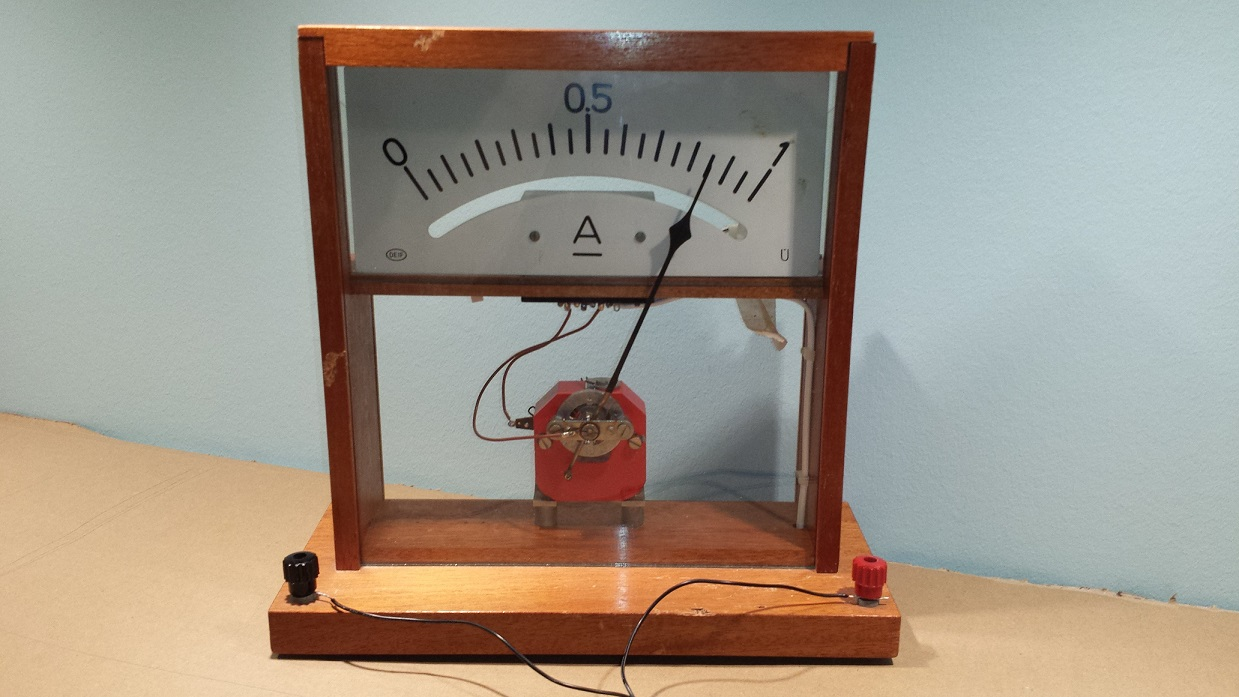
\includegraphics[width=0.6\textwidth]{amperetime}
  \caption{Ampere Time\autocite{amperetime}}
\end{figure}

\framebreak

\begin{figure}[h]
  \centering
  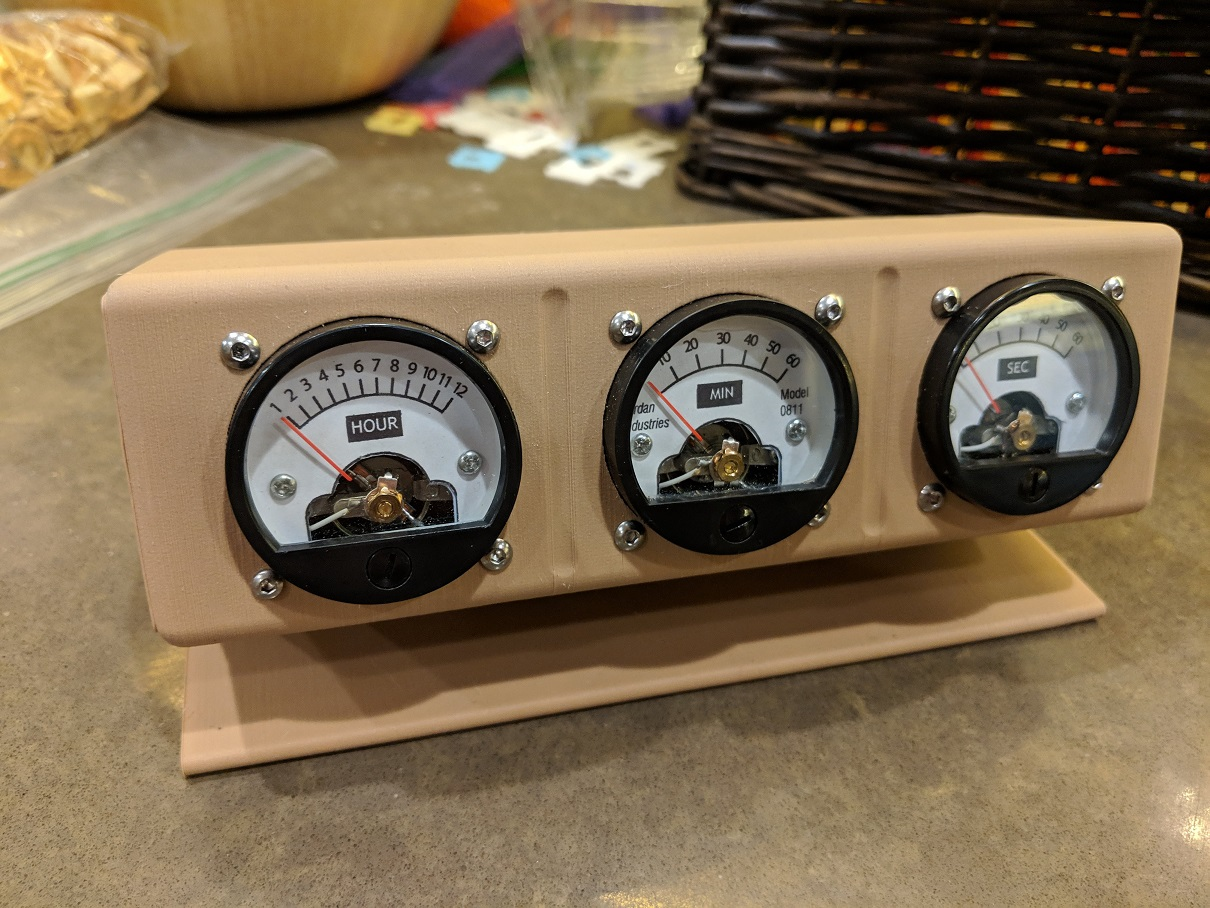
\includegraphics[width=0.4\textwidth]{voltclock}
  \caption{ESP8266 WiFi NTP voltmeter clock\autocite{voltclock}}
\end{figure}
\end{frame}\todo{atrent: idem}


\section{Realizzazione}

\begin{frame}
\frametitle{Analisi delle caratteristiche fisiche degli strumenti}

\begin{figure}[h]
  \centering
  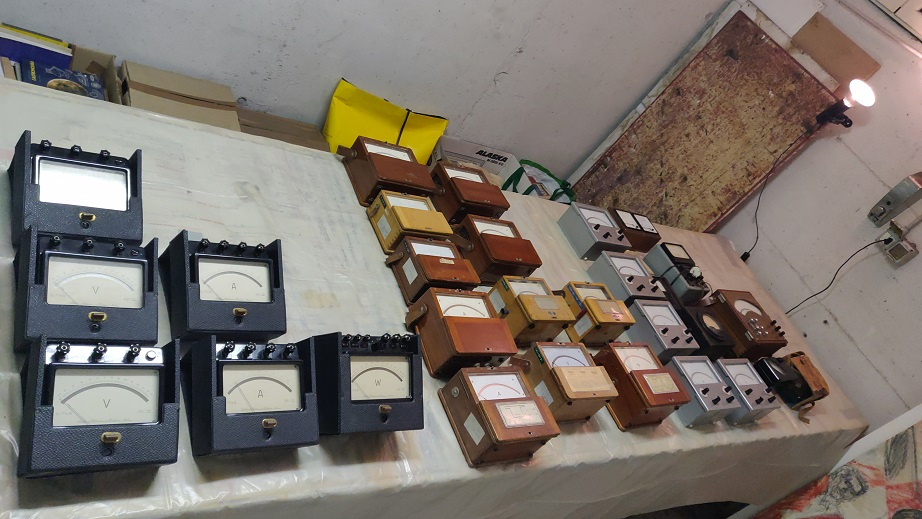
\includegraphics[width=0.7\textwidth]{strumentiago}
  \caption{Strumenti ad ago}
\end{figure}
\end{frame}

\begin{frame}[fragile]
\frametitle{Generalizzazione dei componenti}
\begin{columns}
\column{0.5\textwidth}
\begin{figure}[h]
  \centering
  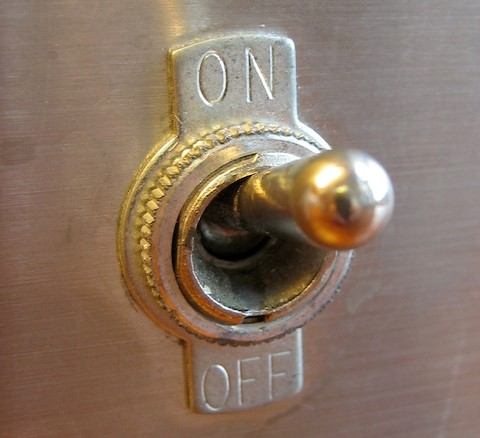
\includegraphics[width=0.6\textwidth]{switch}\footnotemark 
  
\end{figure}

\column{0.5\textwidth}
\begin{lstlisting}[language=cpp]
status = digitalRead(D2);
\end{lstlisting}

\begin{lstlisting}[language=yaml]
binary_sensor:
  - platform: gpio
    pin: D2
    name: "Interruttore"
\end{lstlisting}
\end{columns}
\footcitetext{wiki:switch}
\end{frame}\todo{atrent: invece qui metterei qualche esempio in più (avendo risparmiato slide prima), ad esempio il commutatore}

\begin{frame}
\frametitle{Produzione di una guida alla conversione}
\centering
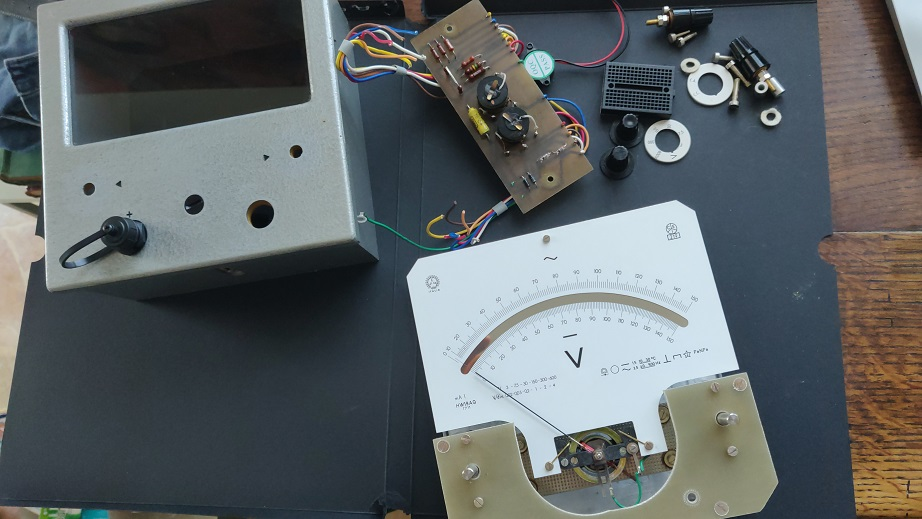
\includegraphics[width=0.45\textwidth]{strumentosmontato}
\enspace
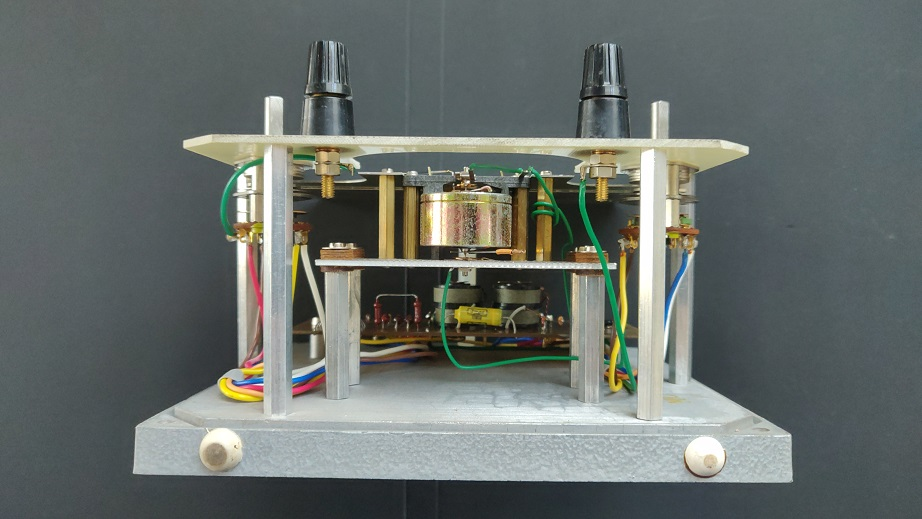
\includegraphics[width=0.45\textwidth]{strumentosenzascocca}
\end{frame}


\begin{frame}[fragile,allowframebreaks]
\frametitle{Il prototipo - IoTDial}
\begin{figure}[h]
  \centering
  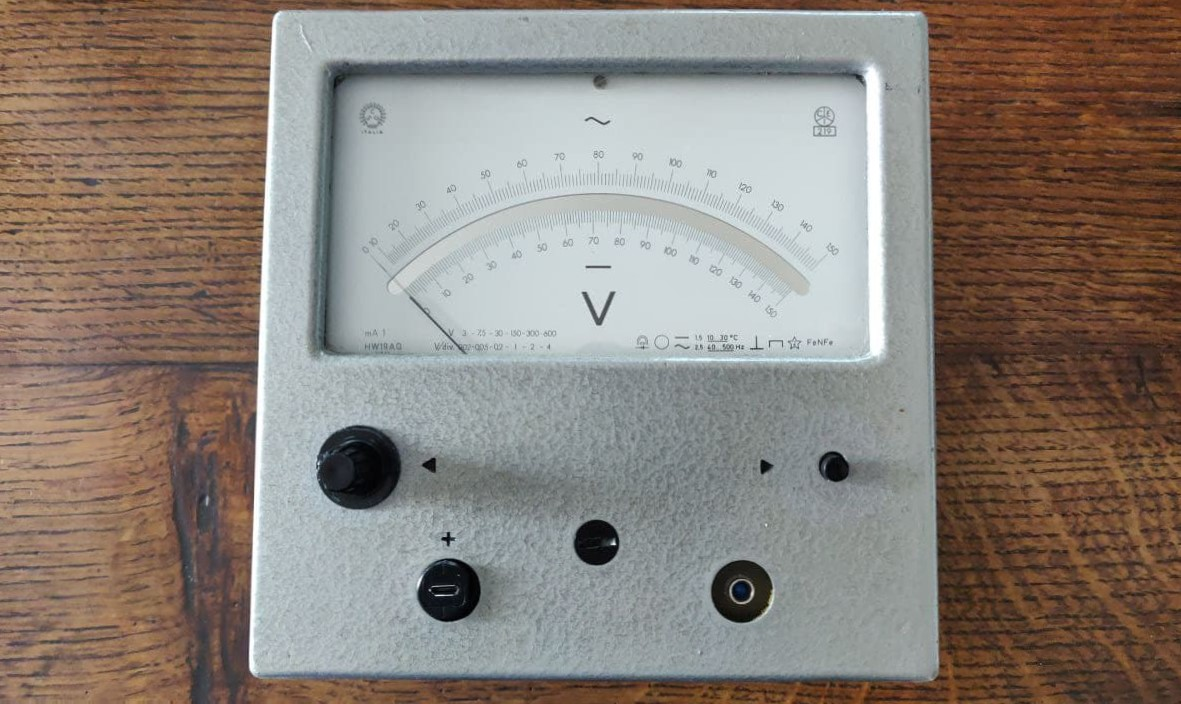
\includegraphics[width=0.65\textwidth]{iotdial}
  \caption{IoTDial}
\end{figure}

\framebreak

\begin{columns}
\column{0.5\textwidth}
Attivo
\begin{lstlisting}[language=cpp]
bool begin;
if (use_https) {
  begin = http.begin(ssl_client, apiUrl);
  Serial.print("[HTTPS] ");
} else {
  begin = http.begin(client, apiUrl);
  Serial.print("[HTTP] ");
}
\end{lstlisting}

\column{0.5\textwidth}
Passivo
\begin{lstlisting}[language=yaml]
esphome:
  name: iotdial-aabbccdd
  platform: ESP8266
  board: d1_mini
  esp8266_restore_from_flash: yes

wifi:
  ssid: !secret wifi_ssid
  password: !secret wifi_password
\end{lstlisting}
\end{columns}
\end{frame}


\section{Conclusioni}
\begin{frame}
\frametitle{Dati}
Quali dati ha senso prelevare e visualizzare?
\vspace{1cm}

Alcuni esempi:
\begin{itemize}
  \item ``Eventi'' (urbani, climatici...)
  %\item Eventi climatici
  \item Statistiche sulla rete locale
  \item Informazioni domestiche, es. temperatura frigo/forno
\end{itemize}
\end{frame}\todo{atrent: parla dei problemi di scraping (specie su esp8266) e della "segretezza" delle API}

\begin{frame}
\frametitle{Feedback}
\begin{figure}[h]
  \centering
  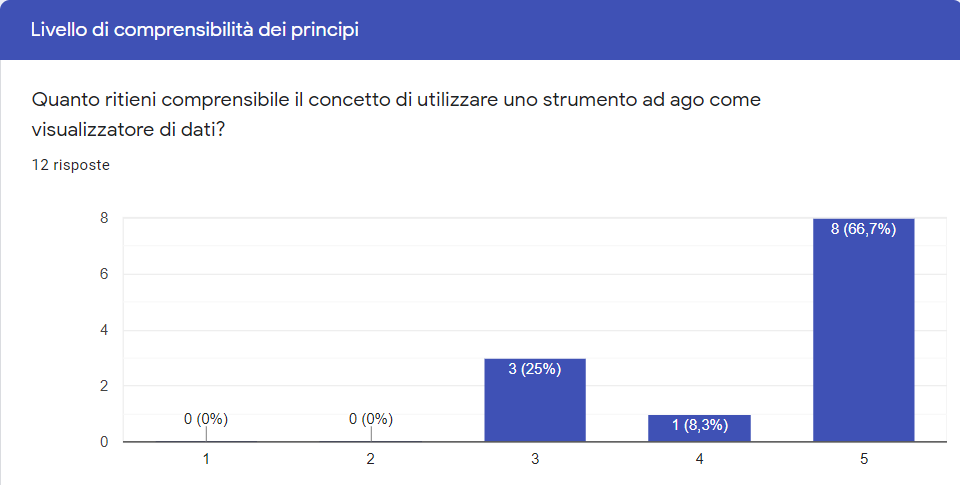
\includegraphics[width=0.7\textwidth]{esempioform}
  \caption{Esempio di risultato della raccolta feedback \footnote{Raccolte impressioni e suggerimenti dai membri dell'HackLab Cormano e dagli studenti dei corsi di Sistemi Embedded e Progettazione di Sistemi Operativi.}}
\end{figure}
\end{frame}\todo{atrent: non è un "esempio del risultato", è il risultato ;)}

\section*{}
\begin{frame}{}
  \centering \Large
  \emph{Fin}
\end{frame}

\end{document}